\documentclass{article}
\usepackage{ocgx}
% Language setting
% Replace `english' with e.g. `spanish' to change the document language
\usepackage[english]{babel}

% Set page size and margins
% Replace `letterpaper' with `a4paper' for UK/EU standard size
\usepackage[letterpaper,top=2cm,bottom=2cm,left=3cm,right=3cm,marginparwidth=1.75cm]{geometry}

% Useful packages
\usepackage{amsmath}
\usepackage{graphicx}
\usepackage[colorlinks=true, allcolors=blue]{hyperref}
\usepackage{tikz}

\title{{Algorithms SV worksheet 5}}
\author{Bálint Molnár}

\begin{document}
\maketitle
 
\emph{I understand that the order in which the topics are taught has changed slightly from previous years. Before attempting the questions, make sure you know the following concepts/definitions: DAG, Minimum Spanning Tree/Kruskal's Algorithm, Max-flow problem/Ford-Fulkerson algorithm, Topological sort, Strongly Connected Components, Bipartite Graph Matching. You may want to use the \href{https://www.cl.cam.ac.uk/teaching/2324/Algorithm1/content/algorithms2.pdf}{notes from 2024.}}

\begin{enumerate}
    \item If we take a DAG and reverse all the edges, do we get a DAG? Briefly justify your answer.

    \item Let $G$ be a weighted graph with positive weights. Show that if you replace all the weights with their squares, the resulting graph has the same Minimum Spanning Tree.

    \item You are given an $N \times N $ grip represented y a matrix $A$ consisting of 0s and 1s. You want to choose $N$ cells in such a way that
    \begin{itemize}
        \item You choose exactly one cell from every row.
        \item You choose exactly one cell from every column.
        \item You can only choose cells where the corresponding entry is $1$.
    \end{itemize}

    How would you find such a set of cells?


    \item You are given a DAG $G=(V,E)$, and a list of special nodes, $[a_1, ..., a_k]$. It is guaranteed that, for all $1 \leq 1 < k$, there is a path from $a_i$ to $a_{i+1}$.

    Design an algorithm that finds a topological sort of $G$ which minimises the ranks for all $a_i$ in the resulting list.


\item Explain how to solve \href{https://cses.fi/problemset/task/1677}{this coding problem} efficiently. Please include the full code in your preferred programming language, along with an explanation of your approach.

\item
You have an island represented by an $N \times M$ grid, with two harbours located on the boundary (either in the first or last row or first or last column). You want to build a border checkpoint line, a set of cells such that any path between the two harbours must pass through at least one checkpoint cell. A path is a sequence of moves between neighbouring cells (left, right, up or down, no diagonal moves). Checkpoints cannot be built on harbour cells. Each cell $(i,j)$ has an associated cost $A[i,j]$ to build a checkpoint. 

Find a set of checkpoints that satisfies the requirements at a minimal cost.

\textbf{Example}

\begin{center}
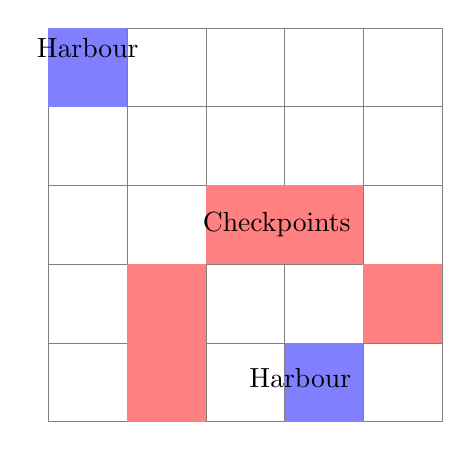
\begin{tikzpicture}
    \draw[step=1cm,gray,very thin] (0,0) grid (5,5);
    
    \foreach \x in {0,...,4} {
        \foreach \y in {0,...,4} {
            \node at (\x+0.5,\y+0.5) {};
        }
    }
    
    % Highlight harbours
    \fill[blue!50] (0,4) rectangle (1,5);
    \fill[blue!50] (3,0) rectangle (4,1);
    
    % Highlight an example checkpoint
    \fill[red!50] (4,1) rectangle (5,2);
    \fill[red!50] (3,2) rectangle (4,3);
    \fill[red!50] (2,2) rectangle (3,3);
    \fill[red!50] (1,1) rectangle (2,2);
    \fill[red!50] (1,0) rectangle (2,1);

    % Labels
    \node[above] at (0.5,4.5) {Harbour};
    \node[below] at (3.2,0.8) {Harbour};
    \node at (2.9,2.5) {Checkpoints};

\end{tikzpicture}
\end{center}
\end{enumerate}
\end{document}